
%*****************************************
\chapter{Case Study}\label{ch:fifth}
%*****************************************

The following chapter presents a user case study which was intended to complement and validate the findings made by Anonymous et al. \cite{anonymous} (see Chapter \ref{ch:third}). The chapter begins by introducing the design of the user case study. Next, the demographic of the recruited participants is presented, followed by a documentation of the study's procedure. Last, the quantitative and qualitative results of the study are discussed. The goal of the research contribution was to examine the effect of \textit{orientation time} on the perceived efficiency of authentication mechanisms. 

\section{Design} \label{5.1}

The user case study was designed as a field study which was conducted in two destinations: on campus of the computer science department at Rheinische Friedrich-Wilhelms-Universit{\"a}t Bonn (Uni Bonn) and at the author's home residence. The independent variable was \textit{ratio} and it had three levels:
\begin{enumerate}
    \item \textcolor{blue}{long} orientation/\textcolor{red}{short} input (abbrv. \textit{long/short}), 
    \item \textcolor{red}{short} orientation/\textcolor{blue}{long} input (abbrv. \textit{short/long}), 
    \item \textcolor{red}{short} orientation/\textcolor{red}{short} input (abbrv. \textit{short/short}). 
\end{enumerate}

The implemented concept \underline{\textbf{FiPa}}, presented in Chapter \ref{ch:forth}, served as a medium to represent the ratios of interest. The order of the ratios was counterbalanced amongst the participants (see figure \ref{fig:permutation}). Data was collected quantitatively by measuring the \textit{orientation} and \textit{input time} for each of the ratios, as explained in Chapter \ref{ch:forth}. Data was also collected qualitatively through a questionnaire, which required study participants to evaluate the aesthetic of the application\footnote{Although this is slightly beyond the scope of the research, I was interested in seeing whether the design of the application had an impact on participants' performance. These observations will be presented later in Chapter \ref{ch:sixth}.}, the ratios (\textit{long/short} and \textit{short/long}), and to also choose which of the two ratios they preferred most. On average, the duration of the study was 20 minutes per participant. 

\section{Participants} \label{5.2}

Twenty-five participants were recruited for the study. Initially, students were informed about the study through a social platform for computer science students at Uni Bonn. Another part was collected on campus of the university's computer science department, and four participants were acquaintances of the author of this thesis. There was no premise for participating in the study, meaning anyone was eligible to partake. Participants who made input-errors (see Section \ref{4.3.2}) were excluded from the evaluation. Nineteen valid data entities remained, of which 13 (62.4\%) were male and 6 (31.6\%) were female. The average age was 21 years, with 17 being the youngest and 31 being the oldest age. The majority of the participants (78.9\%) had an IT-Background and were computer science students. Also, all participants, except for one, used a screen lock for their smartphones: 42.1\% used \textit{Pin}, 36.8\% used \textit{Pattern}, and 15.8\% used \textit{Password} (see figure \ref{fig:demo}). 

\begin{figure}[t!]
\centering
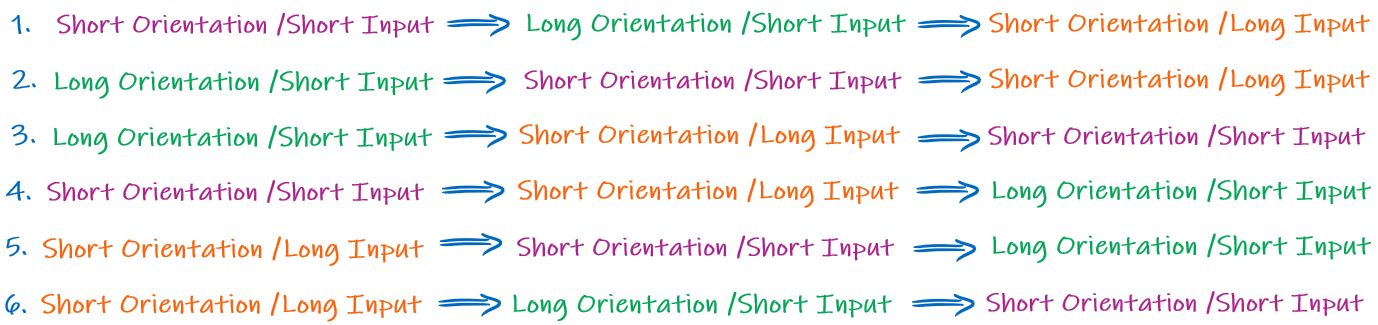
\includegraphics[width=14cm, height=4cm]{Chapters/graphics/permutation.PNG}
\caption{The order in which the three ratios were counterbalanced amongst the participants during the study.}
\label{fig:permutation}
\end{figure}


\section{Procedure} \label{5.3}
The study was held for each participant, separately. First, the experimenter provided a introduction on the study purpose to the participant:

\begin{center}
\textit{Analysis of certain factors of a smartphone authentication process that might play a role in its perceived efficiency.}    
\end{center}

It was also emphasized that the improvement of usability in authentication mechanisms was of interest and that the security aspect was outside the scope of this research study. Moreover, participants were assured that the testing of \underline{\textbf{FiPa}} was not intended to evaluate their cognitive skills or intelligence. It also was important that they felt comfortable and that they did not feel nervous or put under pressure during the course of the study, as it could impact negatively validity of the obtained results.\\

Next, the experimenter described the structure of the application, representing the concept \underline{\textbf{FiPa}}. They explained to the participant that it was meant to emulate an activity, which resembled an authentication concept. They explained the application presented a series of small "challenges", for the participant to solve\footnote{"Challenges"  meant the \textbf{mental} and \textbf{practical tasks}, explained in Chapter \ref{ch:forth}.}. The simple challenges were demonstrated with the help of the paper prototype, shown in figure \ref{fig:paperprototype}.\\

\begin{figure}[t!]
\centering
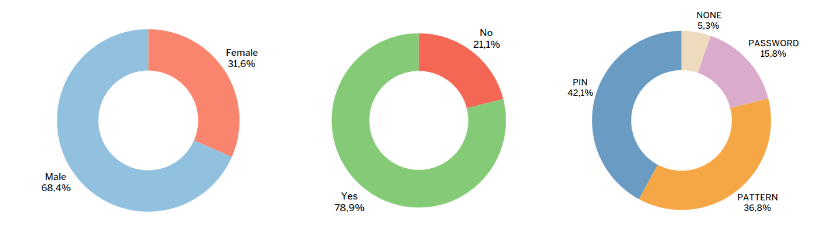
\includegraphics[width=15cm, height=5cm]{Chapters/graphics/Demos.PNG}
\caption{Demographic information on the \textit{gender} (Left), \textit{IT-Background} (Middle), and the \textit{personal screen lock choice} (right) of the recruited participants.}
\label{fig:demo}
\end{figure}

After ensuring that the participant had no further questions, the experimenter proceeded by presenting the application to the participant. The application was installed on an Android smartphone provided by research group of Dr. Emanuel von Zezschwitz.\\
First, the participants were advised to begin with the training-segment of the application, presented in section \ref{4.3.2} (see figure \ref{fig:flow}). The purpose of the training-segment was to ensure that the participant understood the concept of \underline{\textbf{FiPa}} and to reduce the number of errors in the quantitative data set. As mentioned in Section \ref{4.3.2}, the participant was allowed to repeat the training-segment, until they felt ready to start with the actual testing the concept. During the training-segment, the experimenter guided them through the process, when help was needed, and explained certain features, such as the \textit{error-recovery} and the method of input. \\

When the participant felt ready to start the test, the experimenter entered a unique \textit{user-id} for the participant. The experimenter did not intervene, as the participant was executing the actual test of the application. Once the participant was done, they were given a questionnaire to fill out (see Appendix \ref{ch:appendix}). At the end of the study, each participant was compensated with 5 Euros.

\section{Results} \label{5.4}

\begin{figure}[t!]
\centering
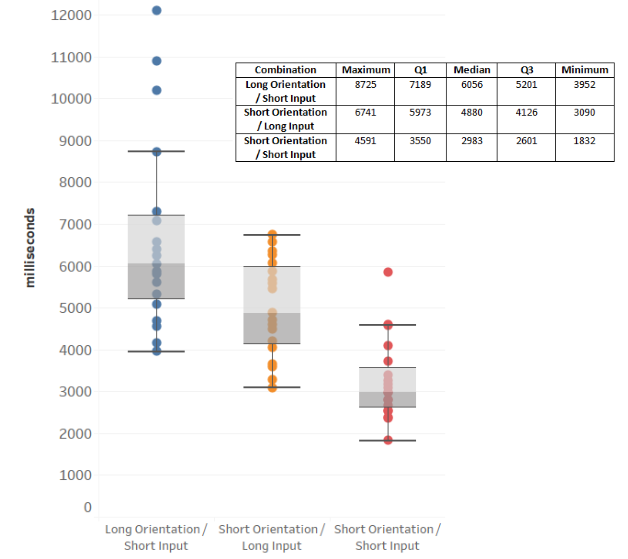
\includegraphics[width=13cm, height=11cm]{Chapters/graphics/Combinations.png}
\caption{A plotted representation of the overall times for each ratio, presented in the study.}
\label{fig:combination}
\end{figure}

\subsection{Measurements}

 As mentioned earlier, \textit{orientation} and \textit{input times} were measured for each ratio. , each \textit{combination} presents three different challenges (couples, see Section \ref{4.2.2.4}). Analogous to the measurement approach, presented in section \ref{4.2.2.4}, the first and second challenge of each combination were considered to be an exercise for the user. Despite the training-segment, participants made a significant amount of mistakes during the first two levels of each phases, and made very little to non in the third. After excluding all data entities which contained unsuccessful input activities, 19 clean data sets remained. \\

Although, the ratios \textit{short/long} and \textit{long/short} (see Section \ref{5.1}) were designed to have the same overall length/duration, results show that they had a temporal difference of 1176 ms, on average (see figure \ref{fig:combination}). The combination \textit{long/short} (6056 ms) had the longest duration, followed by \textit{short/long} (4880 ms) and, lastly, \textit{short/short} (2983 ms) (see figure \ref{fig:combination}). Figure \ref{fig:times} shows that, on average, participants needed notably more time (1094 ms) to finish the long \textit{orientation phase} of \textit{long/short} than they needed for the long \textit{input phase} of \textit{short/long}. If we observe the maximum values of both ratios (see Figure \ref{fig:times}), we notice that one participant needed a maximum time of 9053 ms for long \textit{orientation}. However, the remaining participants' time long \textit{orientation} did not exceed 5202 ms. This implies that for the majority of the time, long \textit{orientation} and long \textit{input} did not significantly differ from each other regarding their measured times. \\
In contrast, the ratios \textit{long/short} and \textit{short/long} differed less notably in terms of the short phases, namely short \textit{orientation} and short \textit{input}. On average, they differed in 572 ms. Nonetheless, participants needed more time for the short \textit{orientation phase} than they needed for the short \textit{input phase} (see figure \ref{fig:times}).

As mentioned earlier in Section \ref{4.1}, the ratio \textit{short/short} was meant to serve as a baseline to the time measurements. By comparing the duration of the phases which \textit{long/short} and \textit{short/long} share with the baseline ratio, it is noticeable that their short \textit{orientation phases} have a difference of 261 ms, whereas the short \textit{input phases} only differ in 2 ms (see figure \ref{fig:times}).  

\begin{figure}[t!]
\centering
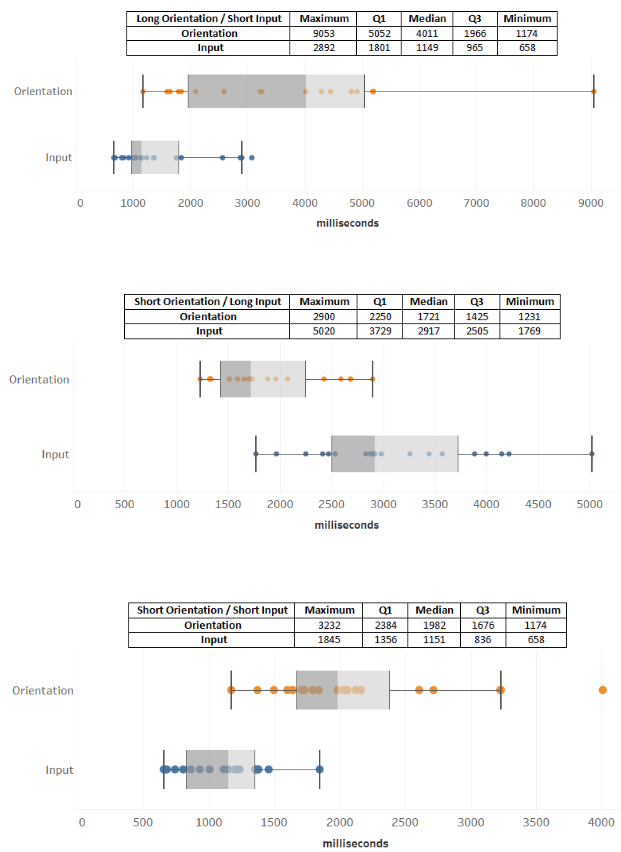
\includegraphics[width=14cm, height=20cm]{Chapters/graphics/Times.png}
\caption{A plotted representation of the time measurements for each ratio, presented in the study: \textit{long/short} (Top);  \textit{short/long} (Middle); \textit{short/short} (Bottom).}
\label{fig:times}
\end{figure}

\subsection{Users' Perception}

A qualitative evaluation of the ratios \textit{long/short} and \textit{short/long} was assessed through a questionnaire (see Appendix \ref{ch:appendix}). As proposed in Section \ref{3.3}, in the questionnaire, the ratios \textit{short/long} and \textit{long/short} were compared to each other, to obtain a precise insight on which of both participants generally preferred more. To ensure the participants had a clear conception of the mentioned ratios, they were given an illustration as an aid to refer to, as they filled out the questionnaire (see figure \ref{fig:illustration}). First, participants were asked to evaluate both ratios separately, through five-point Likert scales (see figure \ref{fig:survey2}, questions 11-12). \\

When participants were asked whether they found the searching process (\textbf{mental task}) of ratio \textit{long/short} annoying, the answers were split between \textit{agree} (8) and \textit{disagree} (8). Three participants found no difference between the two combinations (see figure \ref{fig:likert}). Most participants were able to memorize (89\%) and enter (84\%) the pattern (\textbf{practical task}) easily (see figure \ref{fig:likert}). \\
In contrast, all participants disagreed that the search process \textit{short/long} was annoying. Moreover, all agreed that the pattern was easy to memorize and 89\% agreed that it was easy to enter (see figure \ref{fig:likert}).\\
 
 \begin{figure}[t!]
\centering
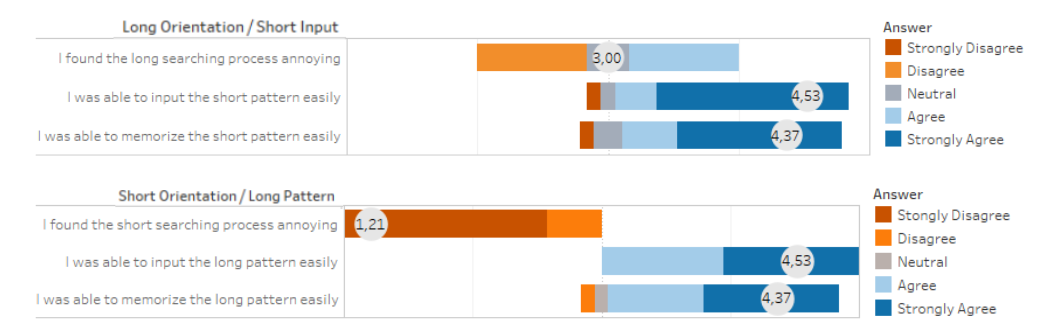
\includegraphics[width=15cm, height=5cm]{Chapters/graphics/Likert1213.PNG}
\caption{A representation of how participants evaluated each ratio separately in terms of this mental and practical task: \textit{long/short} (Top); \textit{short/long} (Bottom).  }
\label{fig:likert}
\end{figure}

Next, participants were asked certain actively choose which ratio they preferred best in terms of certain given characteristics (see figure \ref{fig:likert2}). This evaluation of the ratios was also assessed through Likert scales (see figures \ref{fig:survey2}, \ref{fig:survey3}, questions 13-19). The majority of the participants (68\%) found that \textit{long/short} required more mental effort, about 16\% chose \textit{short/long} and another 16\% saw no difference between both ratios (see figure \ref{fig:likert2}). \\
Moreover, about 79\% voted for \textit{short/long} as the easiest, followed by a 16\% finding \textit{long/short} easier, followed by 5\% who saw no difference between the two (see figure \ref{fig:likert2}). Participants were also asked to chose the ratio, which they found was took longer to find. All participants agreed that the pattern for \textit{long/short} took longer to find (see figure \ref{fig:likert2}). In contrast, participants were asked which pattern they found took longer to enter. Seventy-four percent chose \textit{short/long}, 26\% saw no difference, and 0\% chose \textit{long/short}. Lastly, participants were asked which combination they found was more efficient. The majority 58\% found that \textit{short/long} was more efficient, followed by 26\% chose \textit{long/short}, and 16\% who saw no difference (see figure \ref{fig:likert2}). \\

If we compare the participants' estimation, regarding which ratio had the longest duration, to the actual time measurements, we will find that 36\% (4) misestimated and thought \textit{long/short}, whereas \textit{short/long} was true. Nonetheless the majority of the participants (64\%) estimated correctly. In addition, 18\% percent (2) thought that \textit{short/long} took longer to enter and 36\% (4) didn't perceive a difference, whereas \textit{long/short} was actually true for both cases. Regarding the estimations of the overall duration of the ratios, five participants (26\%) misestimated. In four cases, \textit{long/short} was considered longer, although \textit{short/long} was true. The remaining case found that \textit{long/short}, although the opposite was true. Regarding the estimation for the overall duration of the ratios, three participants found that \textit{short/long} had the longest duration and two participants saw no difference between both ratios, while in actuality \textit{short/long} was true. In addition, one participant misestimated that \textit{long/short} had an overall longer duration.\\

\begin{figure}[t!]
\centering
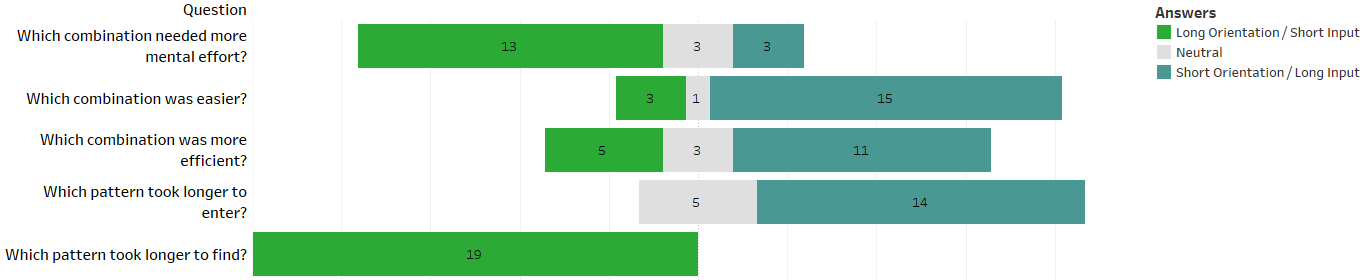
\includegraphics[width=15cm, height=4cm]{Chapters/graphics/Likert2.png}
\caption{Participants were asked to compare the combinations \textit{long/short} and \textit{short/long} to each other by answering the questions above. These questions were answered using Likert scales. }
\label{fig:likert2}
\end{figure}

To get a clearer understanding of the participants' preferences, they were asked to declare which ratio they would prefer for the screen of their smartphone. They were advised to elaborate on their choice based on four given reasons to choose from (see figure \ref{fig:survey3}, question 20): \textit{It's more efficient / more secure / more difficult / challenging}\footnote{Multiple answers were possible.}.\\
Forty-two percent (8) preferred \textit{long/short}, whereas 47\% (9) preferred \textit{short/long} (see figure \ref{fig:preference}). Most frequent reasons given for choosing \textit{long/short} were that is was \textit{more secure} and \textit{more difficult}. Only one participant found that it \textit{more efficient} and only two found that it was \textit{challenging}. Interestingly, one participant elaborated further on their choice and wrote that \textit{short/long} also was more comfortable to use.\\

In contrast, 47\% favored the ratio \textit{short/long} and most frequent reasons given were \textit{more secure} and \textit{more efficient}. The reasons \textit{more difficult} and \textit{challenging} were only given once, each. Two participants elaborated that they would choose \textit{short/long} because it is easier, for when they are tired. Eleven percent (2) chose neither of both ratios and elaborated on their choice in the following (see figure \ref{fig:preference}): 
\begin{itemize}
    \item \textit{"Short/Long is much easier because it's easier to find.\\ It's also much easier to copy => Insecure! I would prefer a mix [of both]."}
    \item \textit{"It don't mind which one, because their use will get easier over time. It really just depends on one's mood."} 
\end{itemize}

\begin{figure}[t!]
\centering
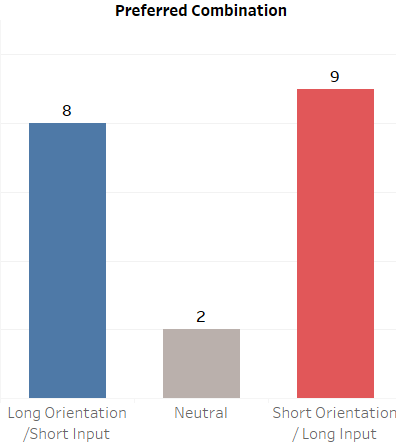
\includegraphics[width=7cm, height=9cm]{Chapters/graphics/preference.png}
\caption{A histogram, representing our participants preferences regarding the combinations.}
\label{fig:preference}
\end{figure}

As mentioned in Section \ref{4.3.2}, a form of \textit{error-recovery} was included into the application with the intention of enhancing its ease-of-use. Although the main focus of our study, was to solely examine certain ratios of \textit{orientation} and \textit{input phases}, it was interesting to find out whether the \textit{error-recovery} feature had an impact on the \textit{orientation time}. For that, a question was added to the survey which only had to be answered if a participant encountered the \textit{error recovery} during the interaction. Answers were assessed through a Likert-scale (see figure \ref{fig:survey3}, question 19). Out of 19 participants, only 6 experienced the \textit{error recovery} (see figure \ref{fig:error})\footnote{We were able to obtain this information during the study, through the database view which was incorporated in the application (see figure \ref{fig:flow}) If a participant had more than three "search-fails", it meant that they encountered the \textit{error-recovery}}. When asked whether the pop-up window feature helped them find the pattern faster, five of the concerned participants agreed and only one disagreed. Moreover, half of the concerned participants (3) disagreed that the pop-up window elongated the searching process. However, one agreed and two answered did not notice any difference. Lastly, when asked whether they found the pop-up window annoying, four disagreed, one agreed, and another was indecisive (see figure \ref{fig:error}). In order to see whether \textit{error-recovery} had an impact on the concerned participants' performance, their quantitative data was examined. Luckily, they never encountered \textit{error-recovery} during the third level of each phase\footnote{As mentioned earlier, the first and second level of each phase in the application, were considered to an exercise. Only the third levels of each phase were involved in the quantitative evaluation.}, which meant that feature had no impact of the measured time. Nonetheless, the examination of the feature's effect still provided information on whether it's design was well accepted by participants. \\

\begin{figure}[t!]
\centering
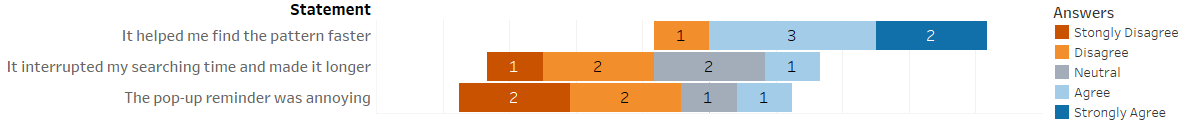
\includegraphics[width=15cm, height=3cm]{Chapters/graphics/ErrorRecovery.png}
\caption{A representation of how participants evaluated the \textit{error-recovery} feature of the application.}
\label{fig:error}
\end{figure}

